\clearpage
\section*{Supporting Information}
\setcounter{section}{0}
\setcounter{table}{0}
\setcounter{figure}{0}
\renewcommand\thetable{SI\arabic{table}}
\renewcommand\thefigure{SI\arabic{figure}}
\section{Additional Details about the Sample and Research Design}

\subsection{Question Wording}
\label{sec:qwording}
\singlespacing
\setlength{\parindent}{0cm} 

\subsubsection{Gun Attitudes and Ownership (Studies 1, 2, and 3)}
Do you favor or oppose a federal law requiring a nationwide ban on people other than law enforcement officers carrying concealed weapons?
\vspace{-3mm}
\begin{itemize}
\setlength\itemsep{-.5em}
  \item Ban people other than law enforcement officers from carrying concealed weapons
  \item Do not ban people other than law enforcement officers from carrying concealed weapons
  \item Unsure
\end{itemize}

How important is the issue to you?
\vspace{-3mm}
\begin{itemize}
\setlength\itemsep{-.5em}
  \item Extremely important
  \item Very important
  \item Somewhat important
  \item Not too important
  \item Not important at all
\end{itemize}

Do you or someone else in your household own a gun?
\vspace{-3mm}
\begin{itemize}
\setlength\itemsep{-.5em}
  \item Yes
  \item No
\end{itemize}

\subsubsection{Minimum Wage Attitudes (Studies 2 and 3 Only)}
The federal minimum wage is currently \$7.25 per hour. Do you favor or oppose raising the federal minimum wage?
\vspace{-3mm}
\begin{itemize}
\setlength\itemsep{-.5em}
  \item Favor raising the federal minimum wage
  \item Oppose raising the federal minimum wage
  \item Neither favor nor oppose raising the federal minimum wage
\end{itemize}

How important is the issue to you?
\vspace{-3mm}
\begin{itemize}
\setlength\itemsep{-.5em}
  \item Extremely important
  \item Very important
  \item Somewhat important
  \item Not too important
  \item Not important at all
\end{itemize}


\subsubsection{Concealed Carry Task (Studies 1, 2, and 3)}
A city government is trying to decide whether to pass a law banning private citizens from carrying concealed handguns in public. Government officials were unsure whether the law would be more likely to decrease crime by reducing the number of people carrying weapons or increase crime by making it harder for law-abiding citizens to defend themselves from violent criminals.

\medskip
Researchers completed a study of two groups of cities to answer that question. The study involved comparing changes in annual crime rates for one group of cities that \uline{had} banned concealed handguns with changes in annual crime rates for a second group of cities that had \uline{not} banned concealed handguns.

\medskip
In each group, the number of cities in which the crime rate \uline{decreased} and the number of cities in which the crime rate \uline{increased} are recorded in the table below. The exact number of cities in each group is not the same, but this does not prevent assessment of the results.

\medskip
\textbf{We would like to know whether cities that enacted a ban were more likely to have a \underline{decrease} or \underline{increase} in crime than cities without bans.}

\begin{table}[h]
\centering
\caption*{{[}Display if randomly assigned to anti-gun condition:{]}} \label{tab:siantigun_corrected}
\begin{tabular}{|l|l|l|}
\hline 
  & Increase in crime  & Decrease in crime \\\hline
  Cities that \underline{did} ban carrying     & \multirow{2}{*}{223 cities} & \multirow{2}{*}{75 cities} \\ 
  concealed handguns in public           &               & \\ \hline
  Cities that \underline{did not} ban carrying & \multirow{2}{*}{107 cities} & \multirow{2}{*}{21 cities} \\ 
  concealed handguns in public           &               &  \\\hline
\end{tabular}
\end{table}

\vspace{-5mm}
\begin{table}[h]
\centering
\caption*{{[}Display if randomly assigned to pro-gun condition:{]}} \label{tab:siprogun_corrected}
\begin{tabular}{|l|l|l|}
\hline 
  & Decrease in crime & Increase in crime \\\hline
  Cities that \underline{did} ban carrying     & \multirow{2}{*}{223 cities} & \multirow{2}{*}{75 cities} \\ 
  concealed handguns in public           &               & \\ \hline
  Cities that \underline{did not} ban carrying & \multirow{2}{*}{107 cities} & \multirow{2}{*}{21 cities} \\ 
  concealed handguns in public           &               &  \\\hline
\end{tabular}
\end{table}

\vspace{-5mm}
\begin{center}
 {[}Page Break{]}
\end{center}

What result does the study support? {[}\textbf{Incentive Treatment:}{]} We will give you a bonus of \$0.10 for the correct answer.
\begin{itemize}
  \item Cities that enacted a ban on carrying concealed handguns were more likely to have \uline{a decrease in crime} than cities without bans.
  \item Cities that enacted a ban on carrying concealed handguns were more likely to have \uline{an increase in crime} than cities without bans.
\end{itemize}

\begin{center}
{[}Page Break{]}\\
\end{center}

On a scale of 0 to 10, where 0 is ``very poorly done'' and 10 is ``very well done,'' how well do you think the study on concealed handguns was done?

\bigskip
On a scale of 0 to 10, where 0 is ``completely unconvincing'' and 10 is ``completely convincing,'' how convincing is this study as evidence of the effect of banning concealed handguns on crime?

\subsubsection{Minimum Wage Task (Studies 2 and 3 Only)}
A city government is trying to decide whether to pass a law increasing the minimum wage. Government officials were unsure whether the law would be more likely to decrease jobs or increase jobs.
 
\medskip
Researchers completed a study of two groups of states to answer that question. The study involved comparing changes in jobs for one group of states that \uline{had} increased the minimum wage with changes in jobs for a second group of states that had \uline{not} increased the minimum wage.
 
\medskip
In each group, the percentage of states in which jobs \uline{decreased} and the percentage of states in which jobs \uline{increased} are recorded in the table below. The exact number of states in each group is not the same, but this does not prevent assessment of the results.
 
\medskip
\textbf{We would like to know whether states that increased the minimum wage were more likely to have a \underline{decrease} or \underline{increase} in jobs than states without minimum wage increases.}

\begin{table}[h]
\centering
\caption*{{[}Display if randomly assigned to pro-raise condition:{]}} \label{tab:siprowage}
\begin{tabular}{|l|l|l|}
\hline 
  & Increase in jobs  & Decrease in jobs \\\hline
  States that \underline{did not} increase     & \multirow{2}{*}{16\%} & \multirow{2}{*}{84\%} \\ 
  minimum wage           &               & \\ \hline
  States that \underline{did} increase & \multirow{2}{*}{37\%} & \multirow{2}{*}{63\%} \\ 
  minimum wage           &               &  \\\hline
\end{tabular}
\end{table}

\vspace{-5mm}
\begin{table}[h]
\centering
\caption*{{[}Display if randomly assigned to anti-raise condition:{]}} \label{tab:siantiwage}
\begin{tabular}{|l|l|l|}
\hline 
  & Increase in jobs  & Decrease in jobs \\\hline
  States that \underline{did} increase     & \multirow{2}{*}{16\%} & \multirow{2}{*}{84\%} \\ 
  minimum wage           &               & \\ \hline
  States that \underline{did not} increase & \multirow{2}{*}{37\%} & \multirow{2}{*}{63\%} \\ 
  minimum wage           &               &  \\\hline
\end{tabular}
\end{table}

\vspace{-2.5mm}
\begin{center}
 {[}Page Break{]}
\end{center}

What result does the study support? {[}\textbf{Incentive Treatment:}{]} We will give you a bonus of \$0.10 for the correct answer.
\begin{itemize}
  \item States that increased the minimum wage were more likely to have \uline{a decrease in jobs} than states without minimum wage increases.
  \item States that increased the minimum wage were more likely to have \uline{an increase in jobs} than states without minimum wage increases.
\end{itemize}

\bigskip
\subsection{Numeracy Screener}
\label{sec:numscreener}
\doublespacing
\setlength{\parindent}{1cm} 

We include our numeracy scale below. It is a shortened version of the scale used by \citet{kahan2017} and developed by \citet{weller2012}. We include the five easiest items that \citeauthor{weller2012} find, in order to identify low-numeracy respondents. Two concerns vitiate commensurability of our scores and those of \citeauthor{kahan2017}: guessing and item sampling. Research suggests that lucky guessing is a minor concern on open-ended items \citep{luskin2011}. And if we assume that the items are Guttman scaled, i.e., a person who answers a more difficult item correctly will also answer easier items correctly, our threshold will be exactly the same as the median score in \citeauthor{kahan2017}. We take Guttman scaling on numeracy items to not only be plausible but likely.

\begin{enumerate}
  \item If we roll a fair, six-sided die 1,000 times, on average, how many times would the die come up as an even number? \\{\bf Answer:} 500
  \item There is a 1\% chance of winning a \$10 prize in the Megabucks Lottery. On average, how many people would win the \$10 prize if 1,000 people each bought a single ticket? \\{\bf Answer:} 10
  \item If the chance of getting a disease is 20 out of 100, this would be the same as having a \underline{\hspace{1cm}}\% chance of getting the disease. \\{\bf Answer:} 20
  \item If there is a 10\% chance of winning a concert ticket, how many people out of 1,000 would be expected to win the ticket? \\{\bf Answer:} 100
  \item In the PCH Sweepstakes, the chances of winning a car are 1 in a 1,000. What percent of PCH Sweepstakes tickets win a car? \\{\bf Answer:} .1
\end{enumerate}

\newpage
\subsection{Respondents Enrolled, Screened, Allocated, and Analyzed by Study}
\label{sec:flow}
Figures~\ref{fig:flowchart1},~\ref{fig:flowchart2}, and~\ref{fig:flowchart3} display source survey counts, released records, observed answers, and policy-position subsets. Counts overlap and are not a sequence of exclusions. Study 1 records include repeated workers; Study 2 records are assumed to represent distinct workers.

\bigskip
\begin{figure}[p]
\centering
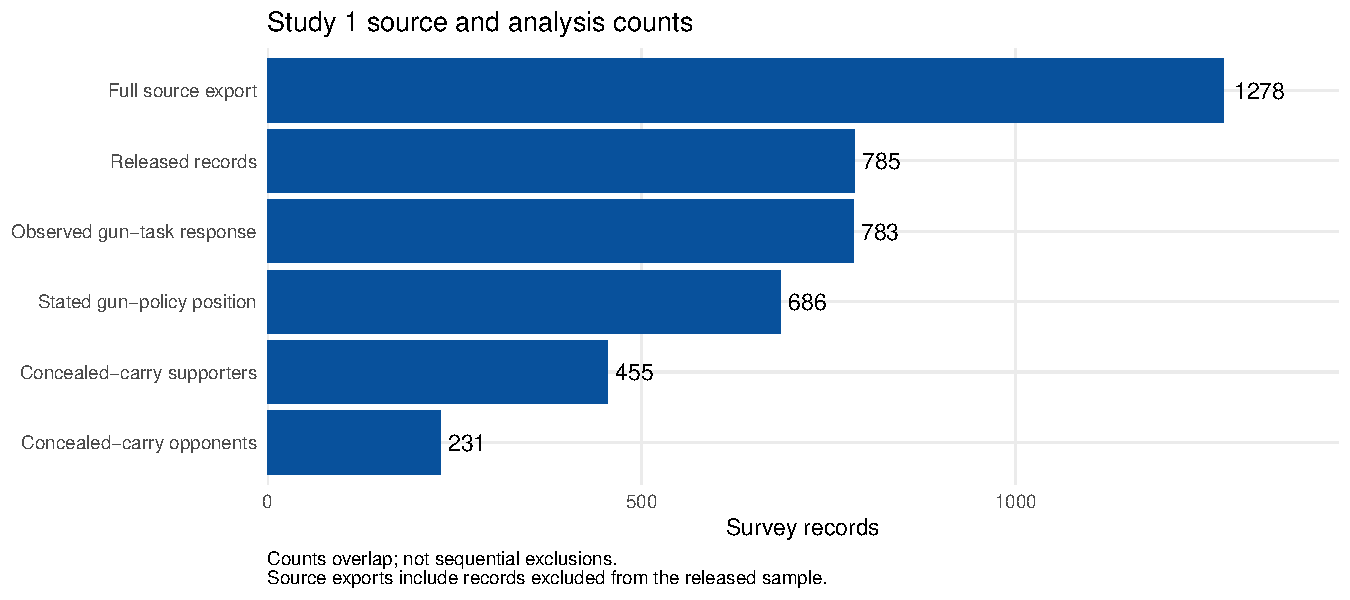
\includegraphics[width=.95\linewidth,height=.34\textheight,keepaspectratio]{../figs/figure_si_1.pdf}
\caption{Study 1 source and analysis counts. Counts overlap; they are not sequential exclusions.}\label{fig:flowchart1}
\end{figure}

\begin{figure}[p]
\centering
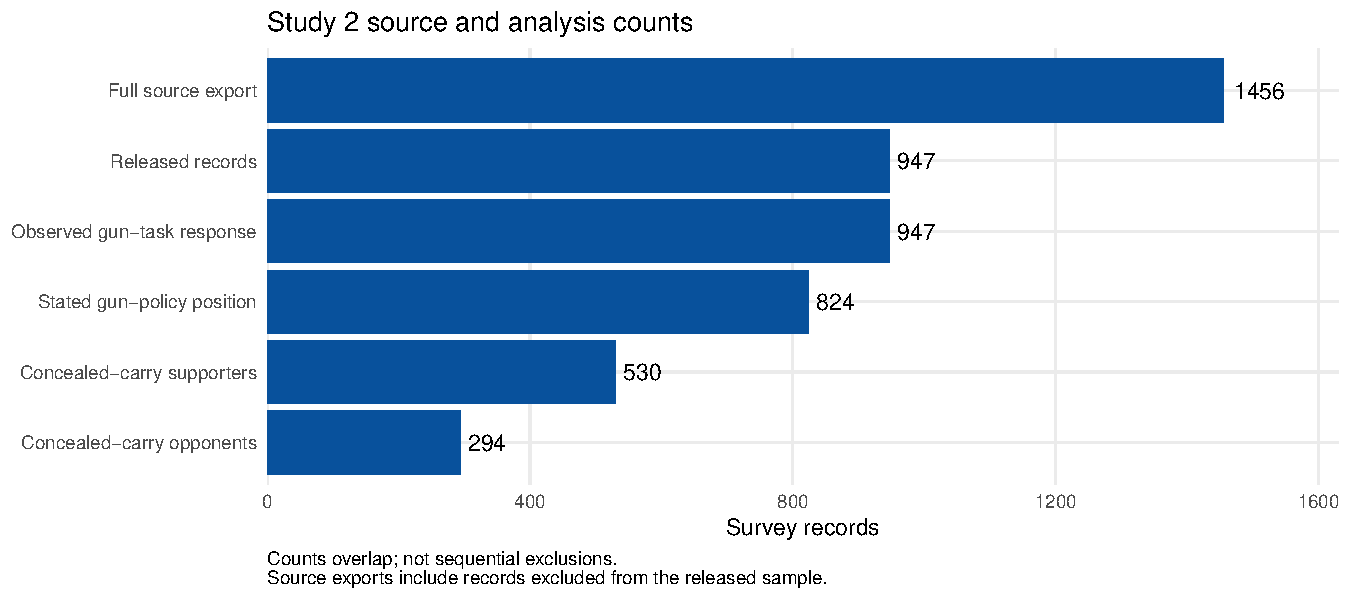
\includegraphics[width=.95\linewidth,height=.34\textheight,keepaspectratio]{../figs/figure_si_2.pdf}
\caption{Study 2 source and analysis counts. Counts overlap; they are not sequential exclusions.}\label{fig:flowchart2}
\end{figure}

\begin{figure}[p]
\centering
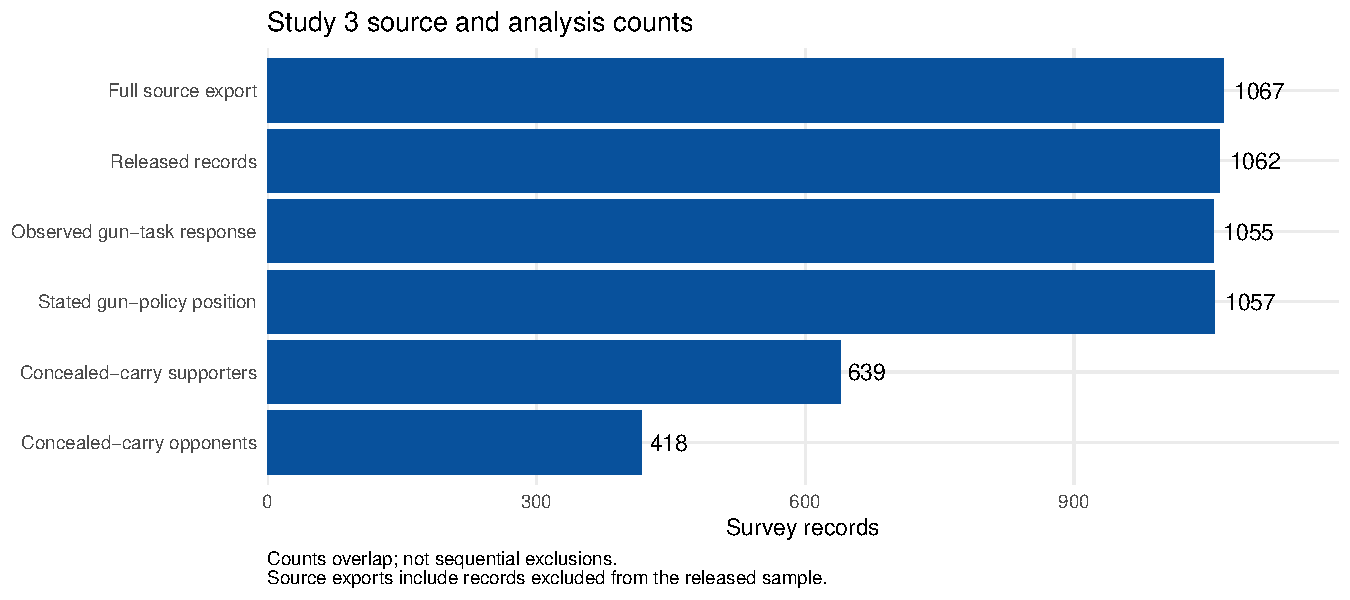
\includegraphics[width=.95\linewidth,height=.34\textheight,keepaspectratio]{../figs/figure_si_3.pdf}
\caption{Study 3 source and analysis counts. Counts overlap; they are not sequential exclusions.}\label{fig:flowchart3}
\end{figure}

\clearpage
\subsection{Sample Characteristics}
\label{sec:sample}

Table~\ref{tab:sample} reports sample characteristics calculated from the reconstructed data. The original supplement also reports national benchmarks from the 2012 American National Election Study and 2015 American Community Survey; those comparisons remain available in the preserved source materials. High numeracy means at least four correct items on the five-item scale. This group contains \result{sample.2.high} records (\result{sample.2.high_pct}\%) in Study 2 and \result{sample.3.high} (\result{sample.3.high_pct}\%) in Study 3. High-numeracy respondents in Study 3 are more educated, white, and male than the full sample.

\singlespacing
\begingroup\footnotesize\singlespacing

\begin{longtable}[t]{lllllll}
\caption{\label{tab:sample}Sample characteristics}\\
\toprule
Characteristic & Category & Study 1 & Study 2 & Study 2: high & Study 3 & Study 3: high\\
\midrule
\endfirsthead
\toprule
Characteristic & Category & Study 1 & Study 2 & Study 2: high & Study 3 & Study 3: high\\
\midrule
\endhead
Party & Democrat & 65.1 (511) & 61.0 (578) & 62.6 (433) & 50.6 (536) & 49.4 (208)\\
Party & Independent & 14.0 (110) & 15.9 (151) & 15.9 (110) & 14.1 (149) & 11.6 (49)\\
Party & Republican & 20.9 (164) & 23.0 (218) & 21.5 (149) & 35.3 (374) & 39.0 (164)\\
Ideology & Conservative & 16.2 (127) & 16.8 (159) & 15.5 (107) & 28.5 (302) & 28.3 (119)\\
Ideology & Liberal & 50.5 (396) & 50.3 (475) & 52.0 (359) & 23.3 (246) & 22.1 (93)\\
Ideology & Moderate & 33.3 (261) & 32.9 (311) & 32.5 (224) & 48.2 (510) & 49.6 (209)\\
Education & College Degree & 39.9 (313) & 38.7 (366) & 39.5 (273) & 26.4 (279) & 33.0 (139)\\
Education & HS or Less & 9.1 (71) & 11.7 (111) & 9.8 (68) & 25.1 (266) & 17.1 (72)\\
Education & Post-Graduate & 10.7 (84) & 8.8 (83) & 10.1 (70) & 9.9 (105) & 13.1 (55)\\
Education & Some College & 40.3 (316) & 40.8 (386) & 40.5 (280) & 38.6 (408) & 36.8 (155)\\
Age & 18-29 & 58.9 (462) & 49.3 (466) & 48.9 (338) & 9.8 (104) & 10.9 (46)\\
Age & 30-44 & 31.5 (247) & 37.7 (357) & 39.5 (273) & 33.9 (358) & 32.5 (137)\\
Age & 45-64 & 9.0 (71) & 11.6 (110) & 10.4 (72) & 43.6 (460) & 46.8 (197)\\
Age & 65 or older & 0.6 (5) & 1.4 (13) & 1.2 (8) & 12.7 (134) & 9.7 (41)\\
Sex & Male & 67.6 (531) & 61.9 (586) & 66.3 (458) & 33.9 (358) & 43.1 (181)\\
Sex & Female & 32.4 (254) & 38.1 (360) & 33.7 (233) & 66.1 (698) & 56.9 (239)\\
Race/ethnicity & Asian, Non-Hisp & 10.6 (83) & 9.5 (90) & 10.9 (75) & 2.9 (30) & 4.1 (17)\\
Race/ethnicity & Black, Non-Hisp & 4.6 (36) & 6.1 (58) & 5.1 (35) & 10.5 (110) & 5.0 (21)\\
Race/ethnicity & Hispanic/Latino & 5.2 (41) & 6.8 (64) & 6.7 (46) & 6.8 (72) & 3.8 (16)\\
Race/ethnicity & Mixed & 3.6 (28) & 3.8 (36) & 3.9 (27) & 2.1 (22) & 1.4 (6)\\
Race/ethnicity & Other, Non-Hisp & 0.6 (5) & 1.2 (11) & 0.7 (5) & 1.3 (14) & 1.2 (5)\\
Race/ethnicity & White, Non-Hisp & 75.4 (590) & 72.6 (686) & 72.8 (502) & 76.4 (804) & 84.4 (353)\\
\bottomrule
\end{longtable}
\noindent\footnotesize Percent of nonmissing responses, with counts in parentheses. High numeracy means at least four correct items.\par\normalsize

\endgroup
\doublespacing

\clearpage
\subsection{Covariate Balance}
\label{sec:balance}

Table~\ref{tab:balance} reports classical F tests for the historical balance specifications. Studies 1 and 2 use congeniality, incentives, and their interaction except for race, which uses incentives alone; Study 3 uses incentives alone. N is the complete-case sample for each model. Alternative race specifications are provided in the replication tables. These comparisons do not establish that randomization was implemented correctly.

\vspace{-3mm}
\singlespacing
\begingroup\footnotesize\singlespacing

\begin{longtable}[t]{rlrrrrl}
\caption{\label{tab:balance}Covariate balance}\\
\toprule
Study & Outcome & N & F & df1 & df2 & p\\
\midrule
\endfirsthead
\toprule
Study & Outcome & N & F & df1 & df2 & p\\
\midrule
\endhead
1 & party id & 686 & 0.44 & 3 & 682 & 0.727\\
1 & ideology & 685 & 0.30 & 3 & 681 & 0.828\\
1 & education code & 685 & 2.42 & 3 & 681 & 0.065\\
1 & age years & 686 & 1.23 & 3 & 682 & 0.297\\
1 & is female & 686 & 1.53 & 3 & 682 & 0.204\\
1 & is white & 783 & 0.64 & 1 & 781 & 0.424\\
2 & party id & 824 & 0.76 & 3 & 820 & 0.519\\
2 & ideology & 822 & 1.29 & 3 & 818 & 0.275\\
2 & education code & 823 & 0.78 & 3 & 819 & 0.505\\
2 & age years & 824 & 0.56 & 3 & 820 & 0.643\\
2 & is female & 823 & 0.47 & 3 & 819 & 0.706\\
2 & is white & 945 & 1.40 & 1 & 943 & 0.238\\
3 & party id & 1055 & 0.08 & 1 & 1053 & 0.784\\
3 & ideology & 1055 & 0.00 & 1 & 1053 & 0.961\\
3 & education code & 1055 & 2.51 & 1 & 1053 & 0.113\\
3 & age years & 1053 & 1.00 & 1 & 1051 & 0.317\\
3 & is female & 1053 & 1.04 & 1 & 1051 & 0.309\\
3 & is white & 1049 & 0.06 & 1 & 1047 & 0.810\\
\bottomrule
\end{longtable}
\noindent\footnotesize Classical F tests. Studies 1 and 2 use policy-congeniality factorials except race, which uses incentives alone. Study 3 uses incentives alone. Alternative race specifications are in race\_balance\_checks.csv.\par\normalsize

\endgroup
\doublespacing

%\clearpage
\vspace{-5mm}
\subsection{Assessing Spillover}
\label{sec:spillover}

Because the concealed carry task always preceded the minimum wage task in Studies 2 and 3, we assess the extent to which randomization in the former task affected behavior in the latter task. We estimate treatment effects in both tasks simultaneously via logistic regression. The outcome variable indicates correctness in the minimum wage task (1 = correct). The regressors are the congeniality treatment, the incentive treatment, and their interaction, in both tasks. We allow the minimum wage treatments to vary by concealed carry condition.

Table~\ref{tab:spillover} displays results for wage supporters in Studies 2 and 3 and opponents in Study 3. The reconstructed Study 2 model has full factorial rank. Sample sizes and coefficients are taken directly from the fitted models. Individual first-task coefficients provide no clear evidence of spillover, but these tests do not establish its absence. Because task order was fixed, they also do not identify the effect of reversing task order.

\medskip
\begingroup\footnotesize\singlespacing

\begin{longtable}[t]{lllrrlrr}
\caption{\label{tab:spillover}Wage correctness and cross-task assignments}\\
\toprule
Model & Term & Covariance & Estimate & SE & p & N & OR\\
\midrule
\endfirsthead
\toprule
Model & Term & Covariance & Estimate & SE & p & N & OR\\
\midrule
\endhead
Wage 2:1 & Intercept & classical & 1.558 & 0.389 & <0.001 & 613 & 4.750\\
Wage 2:1 & GC & classical & 0.611 & 0.656 & 0.351 & 613 & 1.842\\
Wage 2:1 & GI & classical & 0.777 & 0.719 & 0.280 & 613 & 2.175\\
Wage 2:1 & WC & classical & 0.927 & 0.716 & 0.195 & 613 & 2.526\\
Wage 2:1 & WI & classical & 1.045 & 0.830 & 0.208 & 613 & 2.842\\
Wage 2:1 & GC:GI & classical & 0.717 & 1.349 & 0.595 & 613 & 2.049\\
Wage 2:1 & GC:WC & classical & -1.767 & 0.965 & 0.067 & 613 & 0.171\\
Wage 2:1 & GI:WC & classical & -1.443 & 1.035 & 0.163 & 613 & 0.236\\
Wage 2:1 & GC:WI & classical & 0.450 & 1.412 & 0.750 & 613 & 1.568\\
Wage 2:1 & GI:WI & classical & -1.534 & 1.117 & 0.169 & 613 & 0.216\\
Wage 2:1 & WC:WI & classical & -0.667 & 1.256 & 0.595 & 613 & 0.513\\
Wage 2:1 & GC:GI:WC & classical & -0.157 & 1.627 & 0.923 & 613 & 0.855\\
Wage 2:1 & GC:GI:WI & classical & -1.545 & 1.964 & 0.432 & 613 & 0.213\\
Wage 2:1 & GC:WC:WI & classical & -0.735 & 1.789 & 0.681 & 613 & 0.480\\
Wage 2:1 & GI:WC:WI & classical & 1.209 & 1.618 & 0.455 & 613 & 3.352\\
Wage 2:1 & GC:GI:WC:WI & classical & 2.856 & 2.458 & 0.245 & 613 & 17.387\\
Wage 3:0 & Intercept & classical & 0.211 & 0.326 & 0.517 & 369 & 1.235\\
Wage 3:0 & GI & classical & 0.482 & 0.462 & 0.297 & 369 & 1.619\\
Wage 3:0 & WC & classical & 2.519 & 0.679 & <0.001 & 369 & 12.413\\
Wage 3:0 & WI & classical & 0.792 & 0.480 & 0.099 & 369 & 2.208\\
Wage 3:0 & GI:WC & classical & -1.015 & 0.920 & 0.270 & 369 & 0.363\\
Wage 3:0 & GI:WI & classical & -0.846 & 0.647 & 0.191 & 369 & 0.429\\
Wage 3:0 & WC:WI & classical & -1.443 & 0.900 & 0.109 & 369 & 0.236\\
Wage 3:0 & GI:WC:WI & classical & 0.889 & 1.182 & 0.452 & 369 & 2.432\\
Wage 3:1 & Intercept & classical & 1.655 & 0.303 & <0.001 & 683 & 5.231\\
Wage 3:1 & GI & classical & -0.060 & 0.421 & 0.888 & 683 & 0.942\\
Wage 3:1 & WC & classical & -0.961 & 0.376 & 0.011 & 683 & 0.382\\
Wage 3:1 & WI & classical & -0.032 & 0.414 & 0.939 & 683 & 0.969\\
Wage 3:1 & GI:WC & classical & 0.155 & 0.535 & 0.772 & 683 & 1.167\\
Wage 3:1 & GI:WI & classical & -0.032 & 0.577 & 0.956 & 683 & 0.969\\
Wage 3:1 & WC:WI & classical & 0.452 & 0.531 & 0.394 & 683 & 1.572\\
Wage 3:1 & GI:WC:WI & classical & -0.348 & 0.750 & 0.642 & 683 & 0.706\\
\bottomrule
\end{longtable}
\noindent\footnotesize GC/GI: gun congeniality/incentive; WC/WI: wage congeniality/incentive. Models identify study and wage support (1=yes). Coefficients are log odds; OR: odds ratio. Colons denote interactions. N is the fitted complete-case sample.\par\normalsize

\endgroup
\normalsize
\doublespacing

\clearpage
\doublespacing
\section{Additional Empirical Results}

\subsection{Does Numeracy Condition Treatment Effects?}
\label{sec:numeracy}
\doublespacing

We confined Study 1 to high-numeracy respondents based on the theoretical argument and main result of \citet{kahan2017} that polarization only occurs among this group. However, in Studies 2 and 3, we invited all respondents to participate fully, regardless of numeracy, to compare the behavior and background characteristics of high- and low-numeracy respondents. In theory, respondents may differ by numeracy in multiple ways. First, high-numeracy respondents are probably more educated, which we see in Study 3 (see Table~\ref{tab:sample}). Second, they may hold different attitudes. For example, high-numeracy respondents may exhibit greater political sophistication, ideological constraint, party identification, or other traits that predispose them to motivated learning, motivated responding, or both.

Table~\ref{tab:accnum} compares incentive effects in the concealed carry task by study, congeniality, and numeracy. Effects are percentage-point differences between incentive and no-incentive conditions, with two-sided 95\% intervals and fitted sample sizes. Study 1 includes only high-numeracy respondents. Estimated effects vary across groups, but most intervals are wide. In particular, the positive effect among low-numeracy concealed carry opponents in Study 3 does not exclude zero under two-sided inference.

\singlespacing
\begingroup\footnotesize\singlespacing

\begin{longtable}[t]{rllrrllr}
\caption{\label{tab:accnum}Incentive effects by numeracy and congeniality}\\
\toprule
Study & Numeracy & Group & Congenial & Effect & 95\% interval & p & N\\
\midrule
\endfirsthead
\toprule
Study & Numeracy & Group & Congenial & Effect & 95\% interval & p & N\\
\midrule
\endhead
1 & high & Carry opponents & 0 & 9.07 & {}[-8.73, 26.87] & 0.315 & 123\\
1 & high & Carry opponents & 1 & -7.99 & {}[-27.05, 11.06] & 0.407 & 108\\
1 & high & Carry supporters & 0 & -1.51 & {}[-13.87, 10.84] & 0.809 & 248\\
1 & high & Carry supporters & 1 & -3.30 & {}[-16.91, 10.31] & 0.633 & 207\\
2 & all & Carry opponents & 0 & 17.08 & {}[0.91, 33.26] & 0.039 & 146\\
2 & all & Carry opponents & 1 & -0.28 & {}[-16.66, 16.11] & 0.974 & 148\\
2 & all & Carry supporters & 0 & 0.61 & {}[-11.60, 12.81] & 0.922 & 252\\
2 & all & Carry supporters & 1 & 5.86 & {}[-5.98, 17.70] & 0.331 & 278\\
2 & high & Carry opponents & 0 & 25.40 & {}[6.63, 44.16] & 0.008 & 108\\
2 & high & Carry opponents & 1 & 4.01 & {}[-14.60, 22.62] & 0.670 & 117\\
2 & high & Carry supporters & 0 & -4.15 & {}[-18.71, 10.41] & 0.574 & 180\\
2 & high & Carry supporters & 1 & 2.81 & {}[-11.21, 16.82] & 0.693 & 200\\
2 & low & Carry opponents & 0 & -10.14 & {}[-43.50, 23.21] & 0.541 & 38\\
2 & low & Carry opponents & 1 & -14.96 & {}[-53.05, 23.14] & 0.428 & 31\\
2 & low & Carry supporters & 0 & 13.29 & {}[-9.52, 36.09] & 0.249 & 72\\
2 & low & Carry supporters & 1 & 13.29 & {}[-8.96, 35.54] & 0.238 & 78\\
3 & all & Carry opponents & 0 & 6.93 & {}[-1.81, 15.68] & 0.120 & 416\\
3 & all & Carry supporters & 0 & -0.31 & {}[-7.66, 7.03] & 0.933 & 639\\
3 & high & Carry opponents & 0 & 4.45 & {}[-10.58, 19.49] & 0.559 & 159\\
3 & high & Carry supporters & 0 & 2.93 & {}[-8.50, 14.36] & 0.614 & 261\\
3 & low & Carry opponents & 0 & 7.99 & {}[-2.71, 18.69] & 0.143 & 257\\
3 & low & Carry supporters & 0 & -2.41 & {}[-12.04, 7.21] & 0.622 & 378\\
\bottomrule
\end{longtable}
\noindent\footnotesize Effects are percentage points. Two-sided 95\% t intervals; Study 1 worker CR2, otherwise HC2. High numeracy: at least four correct items.\par\normalsize

\endgroup
\doublespacing

Since numeracy is not a prerequisite for understanding which result is more congenial, we also examined the odds of choosing a congenial rather than uncongenial answer among concealed carry opponents. In Study 2, these odds without incentives are \result{odds.study_2_low.carry_opponents.0.response_odds} for low-numeracy respondents and \result{odds.study_2_high.carry_opponents.0.response_odds} for high-numeracy respondents. With incentives, the corresponding odds are \result{odds.study_2_low.carry_opponents.1.response_odds} and \result{odds.study_2_high.carry_opponents.1.response_odds}. These are descriptive odds, not probability differences.

Among Study 3 concealed carry opponents, the odds of choosing a congenial answer fall from \result{odds.study_3_low.carry_opponents.0.response_odds} to \result{odds.study_3_low.carry_opponents.1.response_odds} for low-numeracy respondents, and from \result{odds.study_3_high.carry_opponents.0.response_odds} to \result{odds.study_3_high.carry_opponents.1.response_odds} for high-numeracy respondents. Low-numeracy respondents display greater descriptive response bias in both conditions.

\clearpage
\subsection{Subsetting Respondents by ``Ideological Worldview''}
\label{sec:kahan}
\doublespacing

\citet{kahan2017} operationalize congeniality using respondents' ``ideological worldview'' instead of their position on concealed carry. The authors conceive of ideological worldview as a combination of partisanship and ideology, and measure it by simply multiplying the two. At one end of the scale are ``Conservative Republicans,'' and at the other end, ``Liberal Democrats.'' And while we are skeptical, it is possible that ideological worldview establishes what information is congenial to a respondent, more so than relevant attitudes. To explore this concern, we construct a similar variable, categorizing respondents as either conservative Republicans or liberal Democrats, depending on their self reported party identification (including leaners) and three-point ideology (conservative, moderate, or liberal). Using this variable, we re-analyze the concealed carry task in Study 1 and high-numeracy Study 2.  

Before we present the results, a caveat: positions on concealed carry are only weakly related to ideological worldview, especially among low-numeracy respondents. In Study 2, for example, the correlation is \result{worldview.study_2.high.correlation} among high-numeracy respondents and \result{worldview.study_2.low.correlation} among low-numeracy respondents. In fact, this weak relationship may be why \citeauthor{kahan2017} do not observe bias among low-numeracy respondents. We prefer to subset respondents by their issue position, precisely because the overlap between issue positions and ideological worldview is not 100\%.

We recode congeniality relative to ideological worldview and present the results in Figure~\ref{fig:libdem}. Among conservative Republicans, the congeniality effects are \result{accuracy.figure_si_4.conservative_republican.congeniality_no_incentive.estimate.one} points without incentives and \result{accuracy.figure_si_4.conservative_republican.congeniality_incentive.estimate.one} with incentives. Their difference is \result{accuracy.figure_si_4.conservative_republican.interaction.estimate.one} points (95\% CI \result{accuracy.figure_si_4.conservative_republican.interaction.ci}). Among liberal Democrats, the corresponding effects are \result{accuracy.figure_si_4.liberal_democrat.congeniality_no_incentive.estimate.one} and \result{accuracy.figure_si_4.liberal_democrat.congeniality_incentive.estimate.one} points, with an interaction of \result{accuracy.figure_si_4.liberal_democrat.interaction.estimate.one} (95\% CI \result{accuracy.figure_si_4.liberal_democrat.interaction.ci}). Neither interaction excludes zero. This coding answers a different question from policy congeniality.

\begin{figure}[p]
\centering
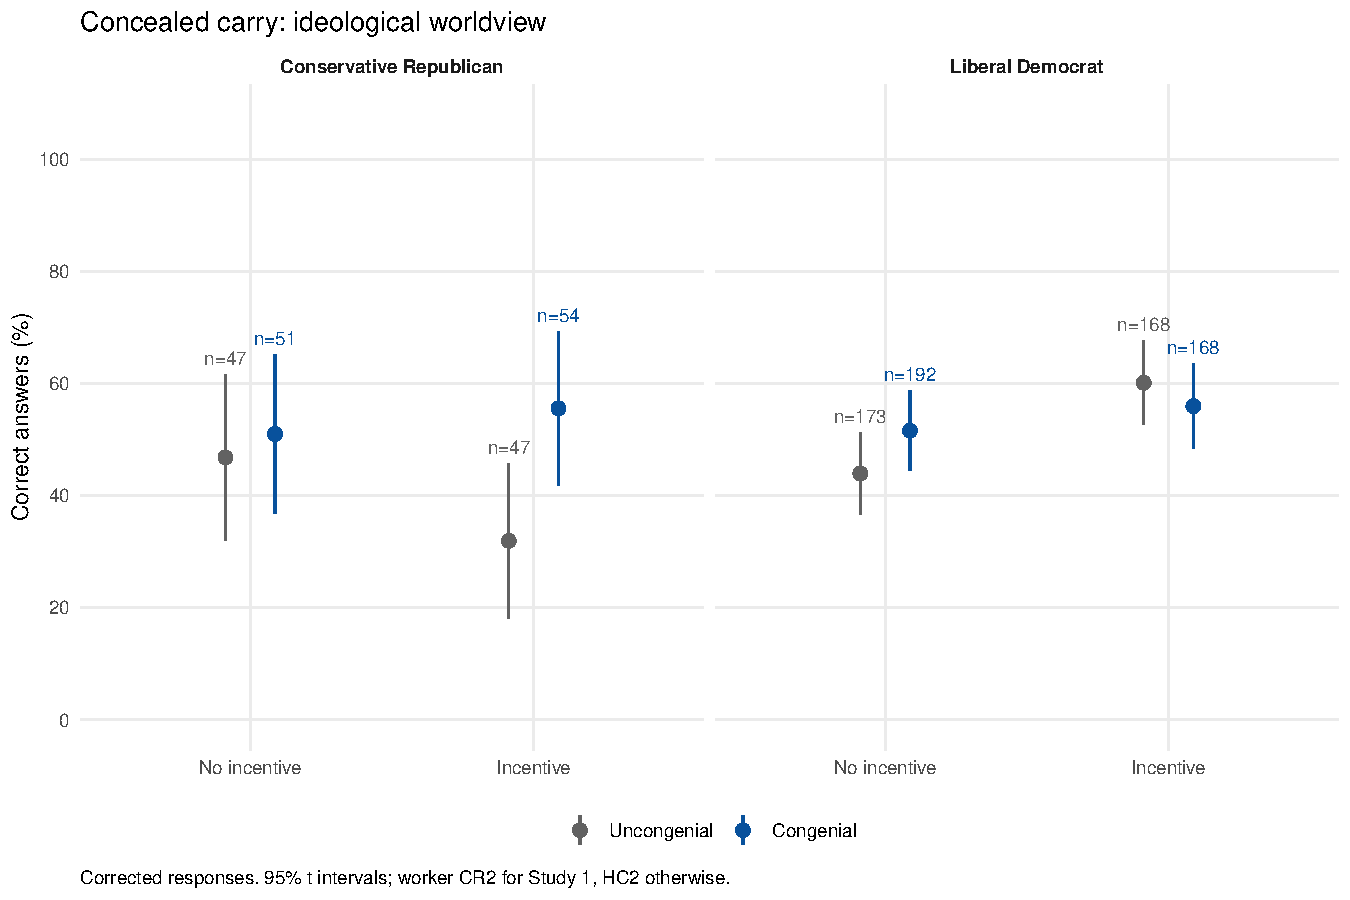
\includegraphics[width=.95\linewidth,height=.34\textheight,keepaspectratio]{../figs/figure_si_4.pdf}
\par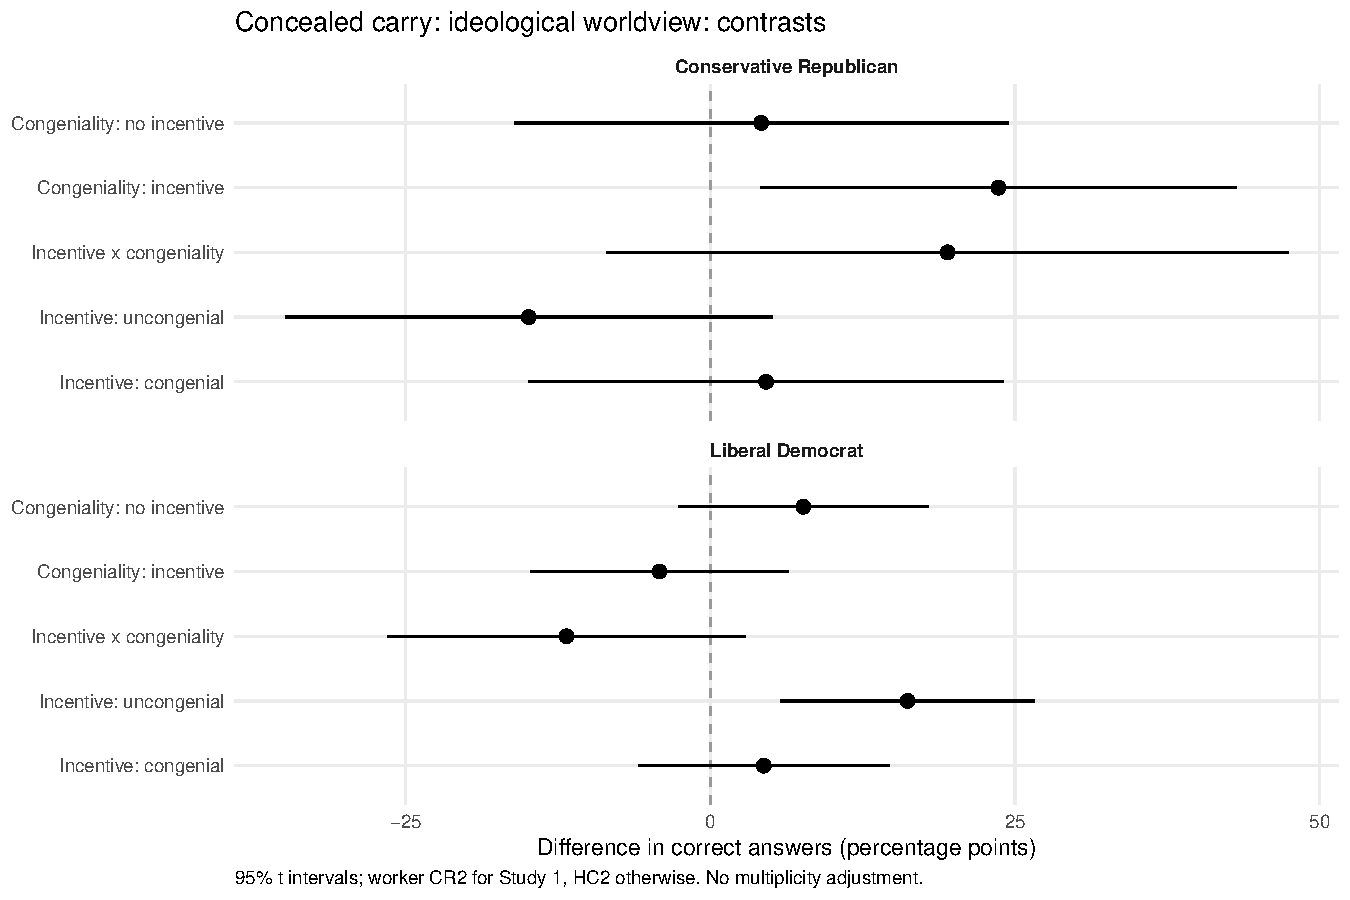
\includegraphics[width=.95\linewidth,height=.34\textheight,keepaspectratio]{../figs/figure_si_4_contrasts.pdf}
\caption{Concealed carry correctness by ideological worldview, Study 1 and high-numeracy Study 2. Upper: correctness by condition. Lower: treatment contrasts. Groups are named in each panel. Intervals are 95\% t intervals, with worker-cluster CR2 for Study 1 samples and HC2 otherwise.}\label{fig:libdem}
\end{figure}

\clearpage
\subsection{Recall of the Stimulus Data}
\label{sec:recall}

One proposed mechanism for why people learn in a motivated manner is that they simply misperceive or misremember the actual data. Thus, we next examine the extent to which errors in cognition are explained by congeniality of the data. Given our hypothesis that motivated responding explains a large portion of what appears to be motivated learning, we also conjectured that most respondents do not perceive data in a selective manner.

To test this hypothesis, we examined how well respondents did across various conditions in recalling the numbers in the contingency table (in Study 1 only). Prior studies using similar tasks suggest that errors are most common in the top-left cell in the contingency table \citep{gilovich1991, dawson2002cella}. We therefore first examine whether the congeniality manipulation changed estimates of the number of cities in this cell. Since the incentive treatment occurred only after respondents saw the contingency table, we do not expect incentives to affect recall. We therefore focus on the effect of congeniality on data recall in the absence of incentives. 

There were always 223 cities in the upper-left cell. If respondents misperceive or misremember this value in a way that makes the study's result more congenial, then we would expect them to overestimate this number in the uncongenial condition, relative to the congenial condition. Overestimating the upper-left cell inflates the crime increase:decrease (decrease:increase) ratio for cities that banned concealed handguns in the anti-gun (pro-gun) version of the table. The estimated mean difference is small. The mean was \result{recall.recall_a.0.estimate.one} (s.e. = \result{recall.recall_a.0.std_error.one}) in the uncongenial condition and \result{recall.recall_a.1.estimate.one} (s.e. = \result{recall.recall_a.1.std_error.one}) in the congenial condition (without incentives).

We next checked whether estimates of the 107 cities in the lower-left cell varied by condition. Here we would expect estimates to be {\it lower} in the uncongenial condition than in the congenial condition. However, recall was again fairly consistent across conditions: \result{recall.recall_c.0.estimate.one} (s.e. = \result{recall.recall_c.0.std_error.one}) and \result{recall.recall_c.1.estimate.one} (s.e. = \result{recall.recall_c.1.std_error.one}) in the uncongenial and congenial conditions, respectively. The other two cells also show no clear congeniality differences. In summary, we do not find a congeniality effect on the recall task in the absence of incentives.

Finally, we estimate the effects of congeniality, incentives, and their interaction on recalled counts. Tables~\ref{tab:recalla} and~\ref{tab:recallc} show classical, HC3, and worker-cluster CR2 uncertainty. The estimates provide no clear evidence of signed recall differences. They do not establish equivalent recall or rule out selective perception, retrieval, or reasoning. These regressions model recalled counts, not absolute recall error.

\vspace{5mm}
\begingroup\footnotesize\singlespacing

\begin{longtable}[t]{lllrrlr}
\caption{\label{tab:recalla}Recall of stimulus cell A}\\
\toprule
Model & Term & Covariance & Estimate & SE & p & N\\
\midrule
\endfirsthead
\toprule
Model & Term & Covariance & Estimate & SE & p & N\\
\midrule
\endhead
Recall a & Intercept & classical & 213.923 & 5.583 & <0.001 & 664\\
Recall a & GC & classical & -1.385 & 8.083 & 0.864 & 664\\
Recall a & GI & classical & -1.918 & 7.974 & 0.810 & 664\\
Recall a & GC:GI & classical & 2.662 & 11.794 & 0.822 & 664\\
Recall a & Intercept & hc3 & 213.923 & 5.547 & <0.001 & 664\\
Recall a & GC & hc3 & -1.385 & 7.417 & 0.852 & 664\\
Recall a & GI & hc3 & -1.918 & 7.663 & 0.802 & 664\\
Recall a & GC:GI & hc3 & 2.662 & 12.169 & 0.827 & 664\\
Recall a & Intercept & cr2 & 213.923 & 5.532 & <0.001 & 664\\
Recall a & GC & cr2 & -1.385 & 7.395 & 0.852 & 664\\
Recall a & GI & cr2 & -1.918 & 7.635 & 0.802 & 664\\
Recall a & GC:GI & cr2 & 2.662 & 12.123 & 0.826 & 664\\
\bottomrule
\end{longtable}
\noindent\footnotesize GC/GI: gun congeniality/incentive. Coefficients are recalled counts. Covariance identifies the inference method. Colons denote interactions. N is the fitted complete-case sample.\par\normalsize

\endgroup

\begingroup\footnotesize\singlespacing

\begin{longtable}[t]{lllrrlr}
\caption{\label{tab:recallc}Recall of stimulus cell C}\\
\toprule
Model & Term & Covariance & Estimate & SE & p & N\\
\midrule
\endfirsthead
\toprule
Model & Term & Covariance & Estimate & SE & p & N\\
\midrule
\endhead
Recall c & Intercept & classical & 103.087 & 3.397 & <0.001 & 665\\
Recall c & GC & classical & 2.099 & 4.910 & 0.669 & 665\\
Recall c & GI & classical & 1.077 & 4.851 & 0.824 & 665\\
Recall c & GC:GI & classical & 1.917 & 7.170 & 0.789 & 665\\
Recall c & Intercept & hc3 & 103.087 & 2.676 & <0.001 & 665\\
Recall c & GC & hc3 & 2.099 & 5.411 & 0.698 & 665\\
Recall c & GI & hc3 & 1.077 & 3.961 & 0.786 & 665\\
Recall c & GC:GI & hc3 & 1.917 & 7.263 & 0.792 & 665\\
Recall c & Intercept & cr2 & 103.087 & 2.668 & <0.001 & 665\\
Recall c & GC & cr2 & 2.099 & 5.396 & 0.697 & 665\\
Recall c & GI & cr2 & 1.077 & 3.952 & 0.785 & 665\\
Recall c & GC:GI & cr2 & 1.917 & 7.232 & 0.791 & 665\\
\bottomrule
\end{longtable}
\noindent\footnotesize GC/GI: gun congeniality/incentive. Coefficients are recalled counts. Covariance identifies the inference method. Colons denote interactions. N is the fitted complete-case sample.\par\normalsize

\endgroup

%\clearpage
\subsection{Covariance Detection Task Results  by Study}
\label{sec:bystudy}

Figures~\ref{fig:study1} and~\ref{fig:study2} separate the concealed carry results by study. Among opponents, the incentive-by-congeniality interactions are \result{accuracy.figure_si_5.carry_opponents.interaction.estimate.one} points in Study 1 (95\% CI \result{accuracy.figure_si_5.carry_opponents.interaction.ci}) and \result{accuracy.figure_si_6.carry_opponents.interaction.estimate.one} points in high-numeracy Study 2 (95\% CI \result{accuracy.figure_si_6.carry_opponents.interaction.ci}). Both intervals include zero.

\begin{figure}[p]
\centering
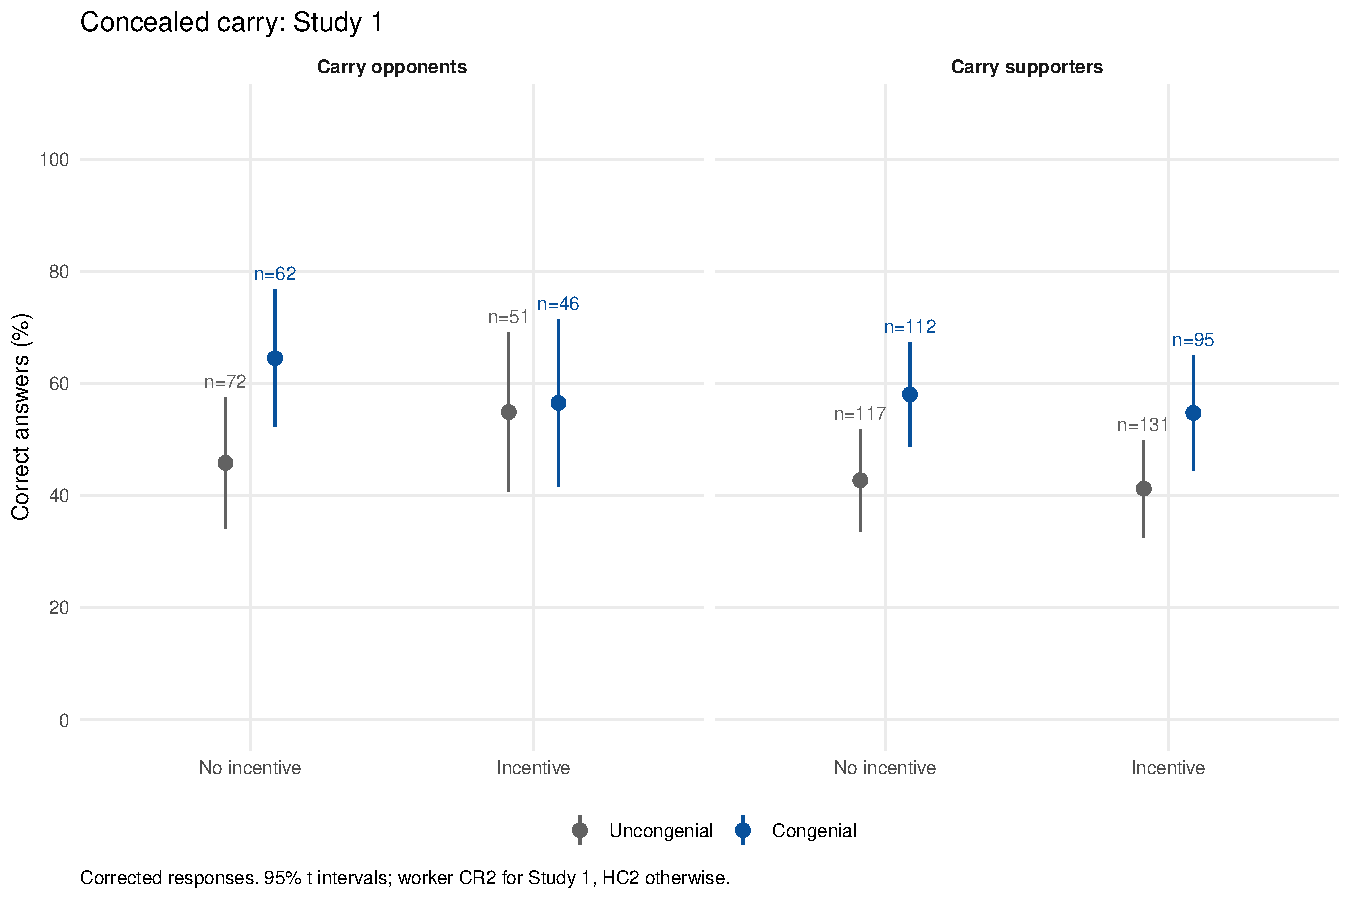
\includegraphics[width=.95\linewidth,height=.34\textheight,keepaspectratio]{../figs/figure_si_5.pdf}
\par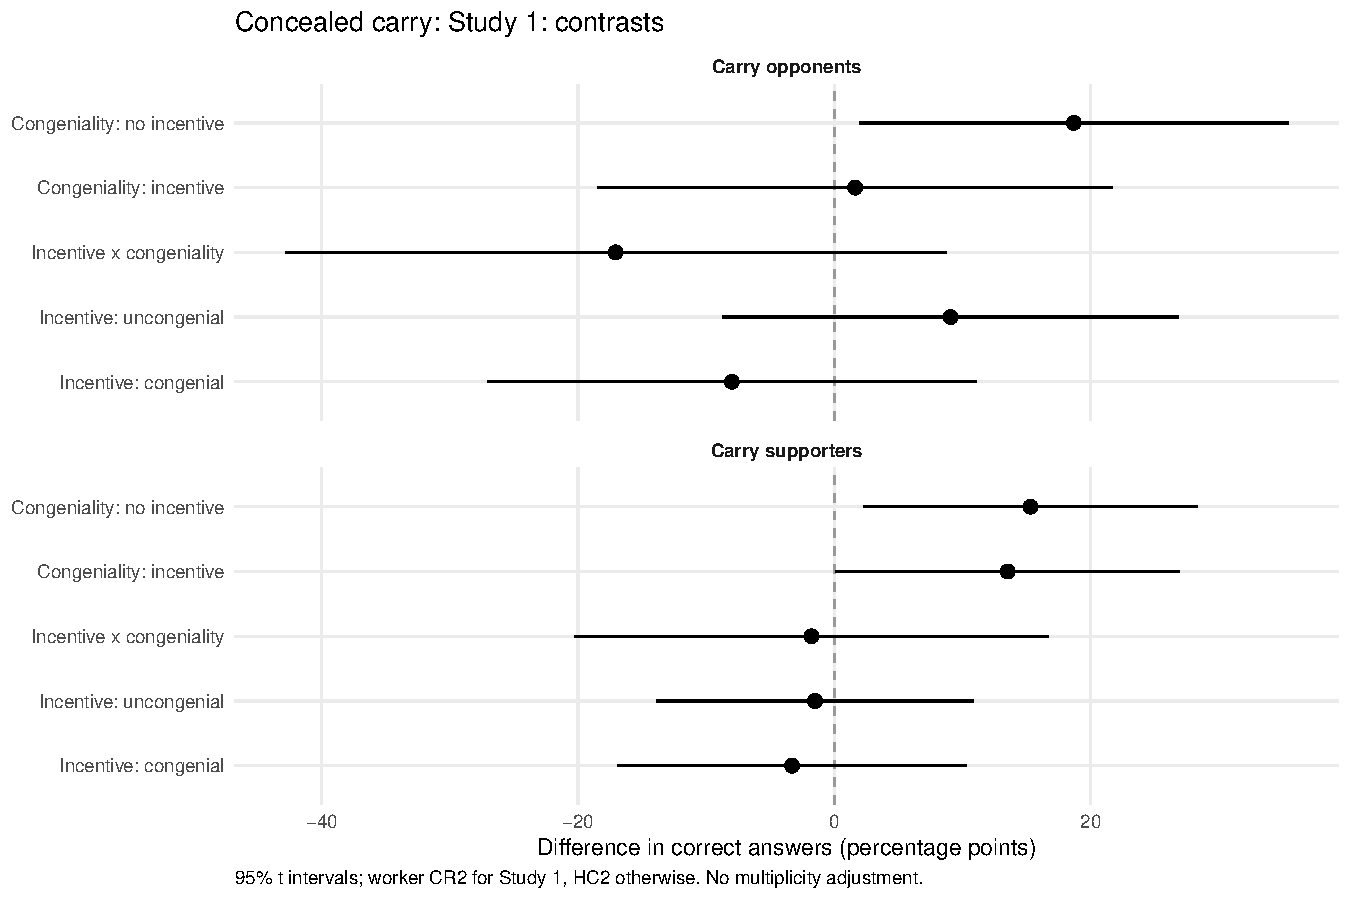
\includegraphics[width=.95\linewidth,height=.34\textheight,keepaspectratio]{../figs/figure_si_5_contrasts.pdf}
\caption{Concealed carry, Study 1. Upper: correctness by condition. Lower: treatment contrasts. Groups are named in each panel. Intervals are 95\% t intervals, with worker-cluster CR2 for Study 1 samples and HC2 otherwise.}\label{fig:study1}
\end{figure}

\begin{figure}[p]
\centering
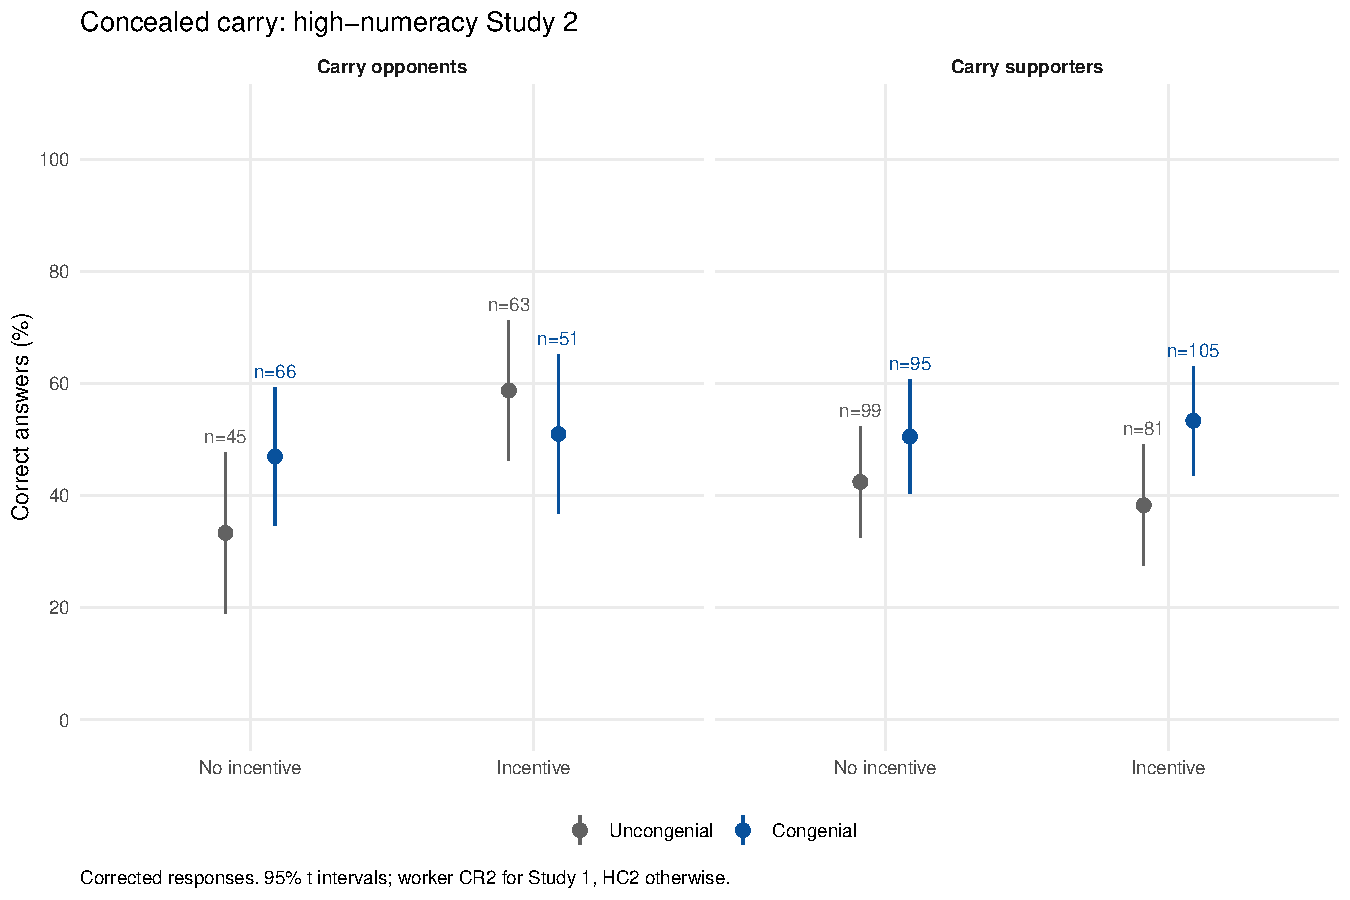
\includegraphics[width=.95\linewidth,height=.34\textheight,keepaspectratio]{../figs/figure_si_6.pdf}
\par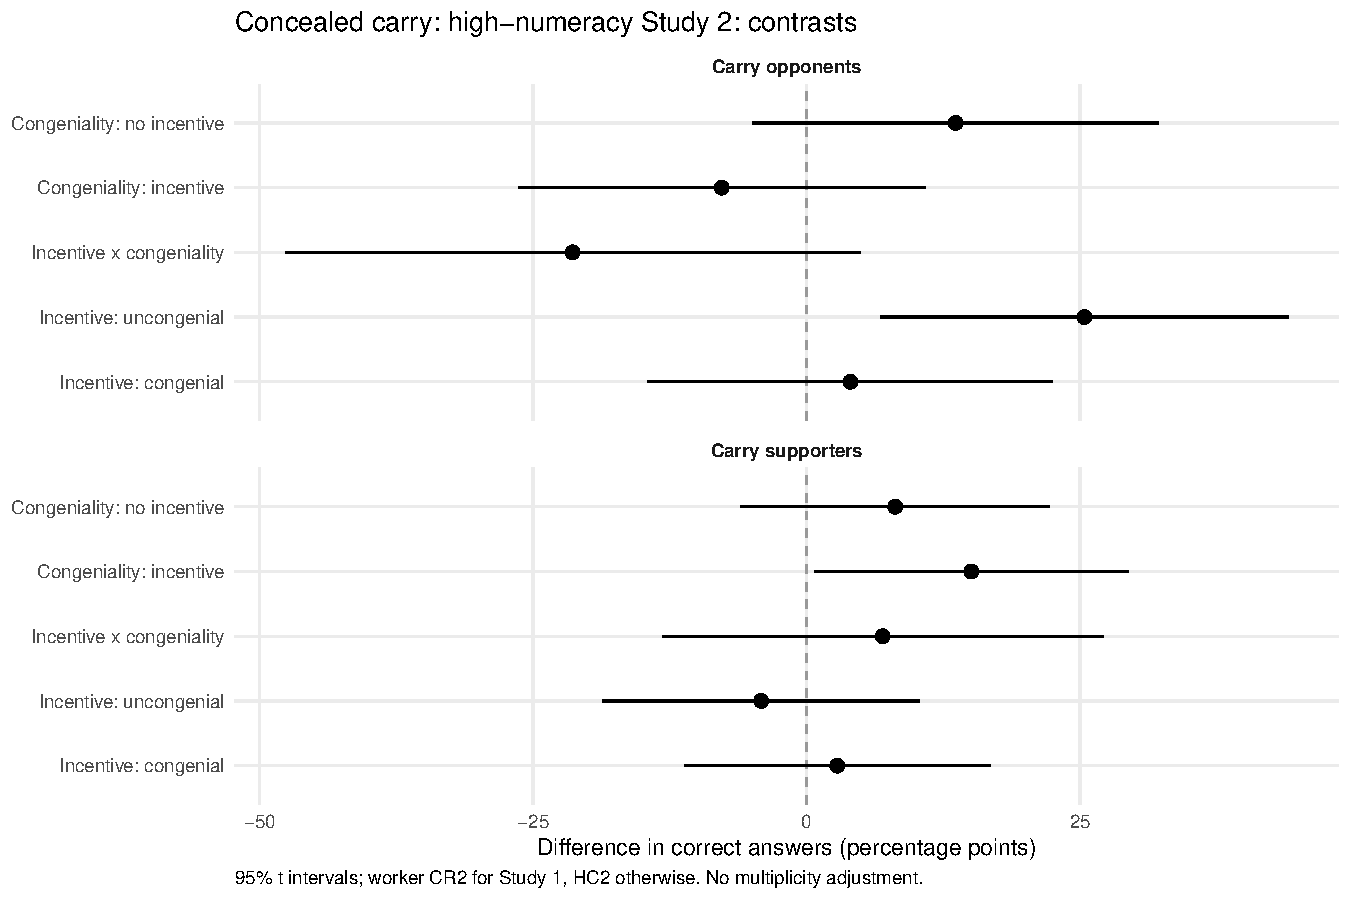
\includegraphics[width=.95\linewidth,height=.34\textheight,keepaspectratio]{../figs/figure_si_6_contrasts.pdf}
\caption{Concealed carry, high-numeracy Study 2. Upper: correctness by condition. Lower: treatment contrasts. Groups are named in each panel. Intervals are 95\% t intervals, with worker-cluster CR2 for Study 1 samples and HC2 otherwise.}\label{fig:study2}
\end{figure}

Figures~\ref{fig:study2_wage} and~\ref{fig:study3_wage} show the minimum wage results separately. Study 2's figure includes wage supporters; Study 3's includes both policy groups. Among Study 3 wage opponents, the interaction is \result{accuracy.figure_si_8.wage_opponents.interaction.estimate.one} points (95\% CI \result{accuracy.figure_si_8.wage_opponents.interaction.ci}; $p\result{accuracy.figure_si_8.wage_opponents.interaction.p}$), so the estimated attenuation remains uncertain.

\begin{figure}[p]
\centering
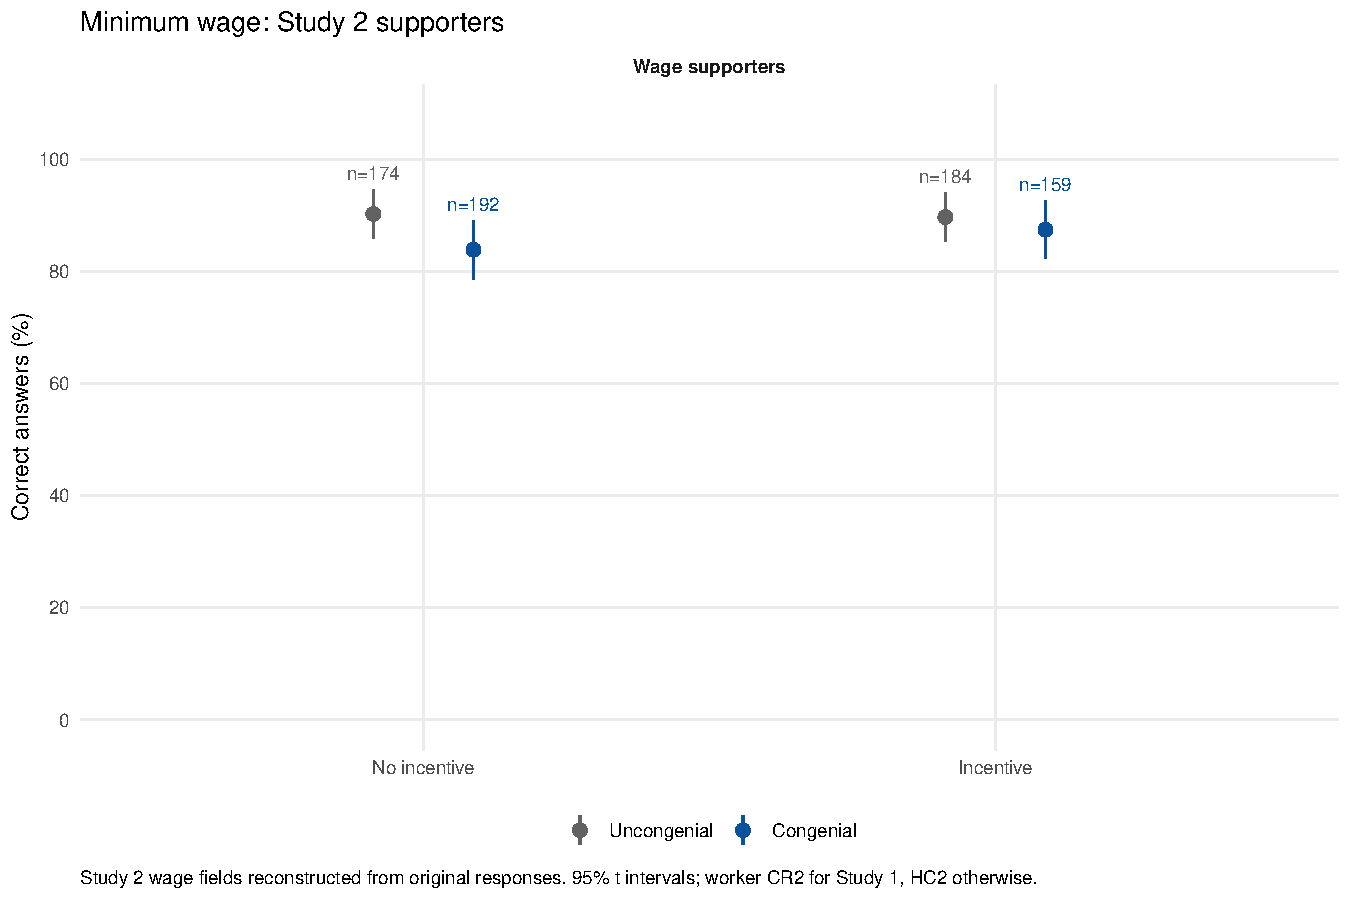
\includegraphics[width=.95\linewidth,height=.34\textheight,keepaspectratio]{../figs/figure_si_7.pdf}
\par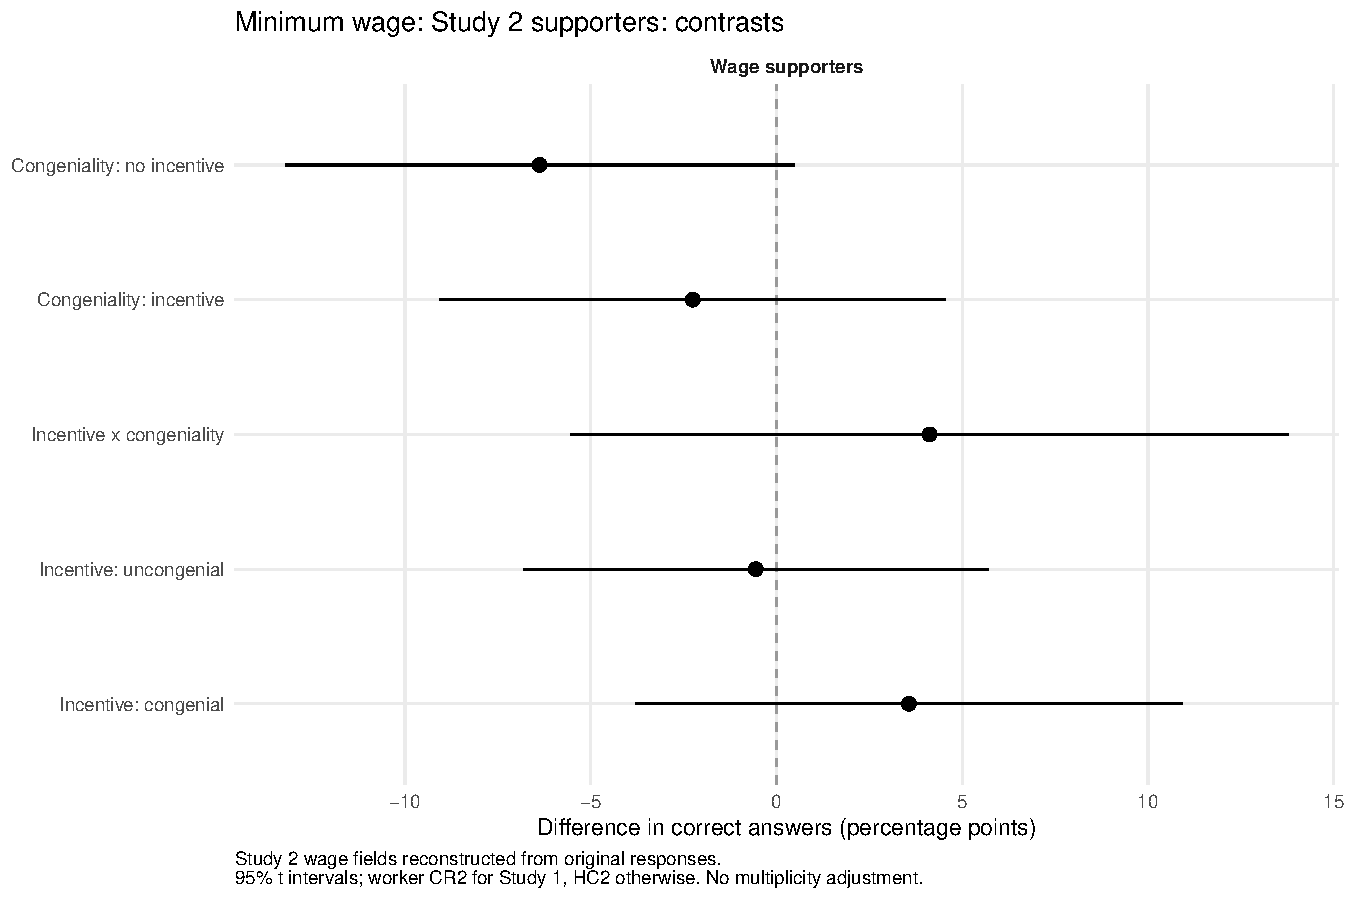
\includegraphics[width=.95\linewidth,height=.34\textheight,keepaspectratio]{../figs/figure_si_7_contrasts.pdf}
\caption{Minimum wage, Study 2 supporters. Upper: correctness by condition. Lower: treatment contrasts. Groups are named in each panel. Intervals are 95\% t intervals, with worker-cluster CR2 for Study 1 samples and HC2 otherwise.}\label{fig:study2_wage}
\end{figure}

\begin{figure}[p]
\centering
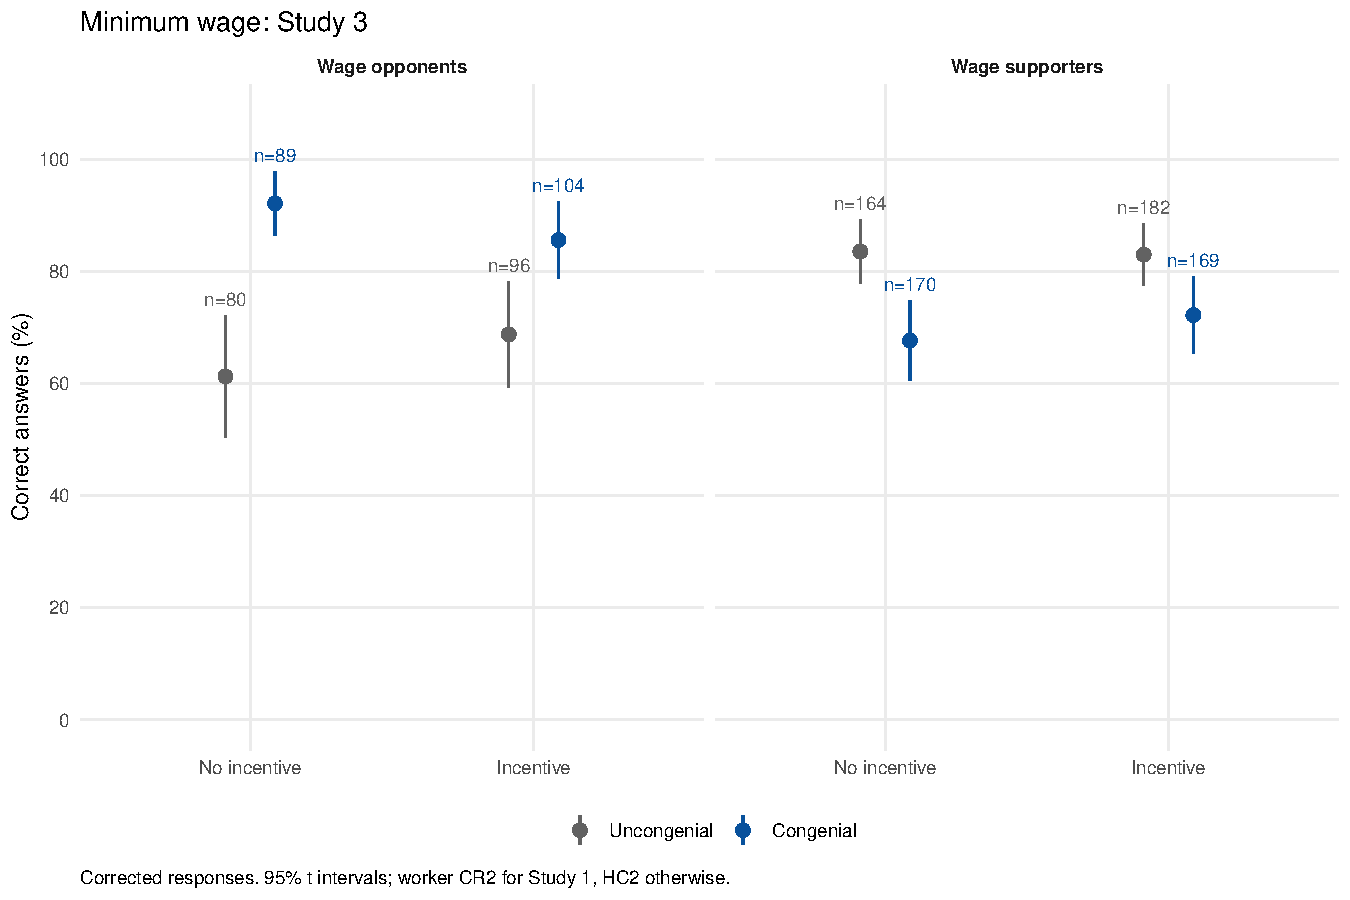
\includegraphics[width=.95\linewidth,height=.34\textheight,keepaspectratio]{../figs/figure_si_8.pdf}
\par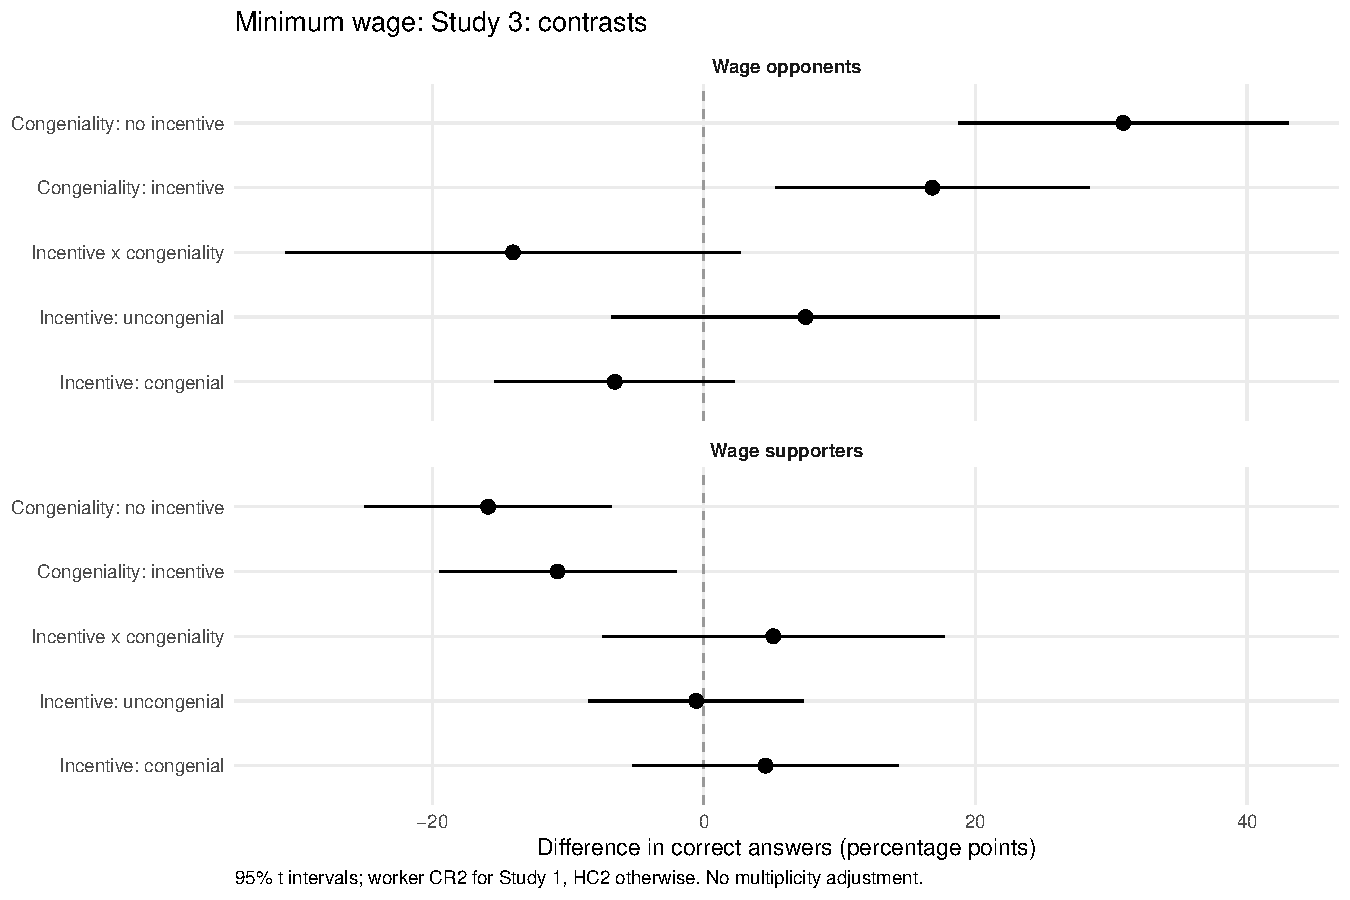
\includegraphics[width=.95\linewidth,height=.34\textheight,keepaspectratio]{../figs/figure_si_8_contrasts.pdf}
\caption{Minimum wage, Study 3. Upper: correctness by condition. Lower: treatment contrasts. Groups are named in each panel. Intervals are 95\% t intervals, with worker-cluster CR2 for Study 1 samples and HC2 otherwise.}\label{fig:study3_wage}
\end{figure}


\clearpage
\subsection{Concealed Carry Task Results as Logistic Regressions}
\label{sec:logit}
\doublespacing

Tables~\ref{tab:logit1} and~\ref{tab:logit2} report logistic specifications for concealed carry supporters and opponents, pooling Study 1 and high-numeracy Study 2. Coefficients are log odds; odds ratios and complete-case N are also shown. These tables retain classical model-based inference for comparison; primary probability contrasts use worker-cluster CR2. The opponent interaction is negative, but the classical two-sided test does not establish a reduction at the .05 level ($p\result{model.gun_logit_position_1.classical.gun_congenial_gun_incentive.p}$).

\bigskip
\begingroup\footnotesize\singlespacing

\begin{longtable}[t]{lllrrlrr}
\caption{\label{tab:logit1}Gun correctness: carry supporters}\\
\toprule
Model & Term & Covariance & Estimate & SE & p & N & OR\\
\midrule
\endfirsthead
\toprule
Model & Term & Covariance & Estimate & SE & p & N & OR\\
\midrule
\endhead
Gun 0 & Intercept & classical & -0.298 & 0.138 & 0.030 & 835 & 0.742\\
Gun 0 & GC & classical & 0.483 & 0.196 & 0.014 & 835 & 1.620\\
Gun 0 & GI & classical & -0.103 & 0.196 & 0.600 & 835 & 0.902\\
Gun 0 & GC:GI & classical & 0.079 & 0.280 & 0.777 & 835 & 1.083\\
\bottomrule
\end{longtable}
\noindent\footnotesize GC/GI: gun congeniality/incentive. Model: ban support (1=yes). Coefficients: log odds; OR: odds ratio. Colons denote interactions. N is the fitted complete-case sample.\par\normalsize

\endgroup
\normalsize
\doublespacing

\begingroup\footnotesize\singlespacing

\begin{longtable}[t]{lllrrlrr}
\caption{\label{tab:logit2}Gun correctness: carry opponents}\\
\toprule
Model & Term & Covariance & Estimate & SE & p & N & OR\\
\midrule
\endfirsthead
\toprule
Model & Term & Covariance & Estimate & SE & p & N & OR\\
\midrule
\endhead
Gun 1 & Intercept & classical & -0.363 & 0.188 & 0.054 & 456 & 0.696\\
Gun 1 & GC & classical & 0.583 & 0.259 & 0.024 & 456 & 1.791\\
Gun 1 & GI & classical & 0.645 & 0.267 & 0.016 & 456 & 1.907\\
Gun 1 & GC:GI & classical & -0.721 & 0.380 & 0.058 & 456 & 0.486\\
\bottomrule
\end{longtable}
\noindent\footnotesize GC/GI: gun congeniality/incentive. Model: ban support (1=yes). Coefficients: log odds; OR: odds ratio. Colons denote interactions. N is the fitted complete-case sample.\par\normalsize

\endgroup
\normalsize
\doublespacing


\clearpage
\subsection{Assessing Experimenter Demand Effects}
\label{sec:demand}

To earn a little extra money, do respondents report what they think the experimenter believes is true instead of what they believe to be true? To answer that, we need to conjecture about respondents' beliefs about the experimenter conducting the study. We consider two hypotheses about what respondents may think in this regard. The first is that respondents believe that most social scientists are liberal, and therefore infer that the result favoring gun control will always be treated as correct. Another is that respondents interpret financial incentives as a cue that the uncongenial option is the right one. We investigate both possibilities.

If respondents believe the experimenter is liberal, incentives should encourage selection of the anti-gun answer regardless of the data. Table~\ref{tab:demand_opp} reports observed answer directions among concealed carry opponents. In the uncongenial condition, incentives reduce the share choosing the congenial anti-gun answer. This pattern conflicts with that simple prediction. Unanswered items are excluded from these response-direction tables rather than assigned an inferred answer.

Among concealed carry supporters, the observed shares choosing the congenial answer are similar across incentive conditions (Table~\ref{tab:demand_supp}). These descriptive comparisons do not establish that incentives have exactly zero effect.

\singlespacing
\begingroup\footnotesize\singlespacing

\begin{longtable}[t]{lrrrrr}
\caption{\label{tab:demand_opp}Reported answer direction: carry opponents}\\
\toprule
Sample & Incentive & Congenial & Congenial answer (\%) & Odds & N\\
\midrule
\endfirsthead
\toprule
Sample & Incentive & Congenial & Congenial answer (\%) & Odds & N\\
\midrule
\endhead
pooled 1 2 & 0 & 0 & 59.0 & 1.44 & 117\\
pooled 1 2 & 0 & 1 & 55.9 & 1.27 & 127\\
pooled 1 2 & 1 & 0 & 43.0 & 0.75 & 114\\
pooled 1 2 & 1 & 1 & 53.6 & 1.16 & 97\\
\bottomrule
\end{longtable}
\noindent\footnotesize Shares are within the specified treatment cell. Odds are congenial answers divided by uncongenial answers.\par\normalsize

\endgroup
\doublespacing

\singlespacing
\begingroup\footnotesize\singlespacing

\begin{longtable}[t]{lrrrrr}
\caption{\label{tab:demand_supp}Reported answer direction: carry supporters}\\
\toprule
Sample & Incentive & Congenial & Congenial answer (\%) & Odds & N\\
\midrule
\endfirsthead
\toprule
Sample & Incentive & Congenial & Congenial answer (\%) & Odds & N\\
\midrule
\endhead
pooled 1 2 & 0 & 0 & 57.2 & 1.34 & 215\\
pooled 1 2 & 0 & 1 & 54.6 & 1.20 & 207\\
pooled 1 2 & 1 & 0 & 59.9 & 1.49 & 212\\
pooled 1 2 & 1 & 1 & 54.0 & 1.17 & 200\\
\bottomrule
\end{longtable}
\noindent\footnotesize Shares are within the specified treatment cell. Odds are congenial answers divided by uncongenial answers.\par\normalsize

\endgroup
\doublespacing

Do respondents interpret the incentive as a cue that the uncongenial answer is correct regardless of the data? The patterns in Tables~\ref{tab:demand_opp} and~\ref{tab:demand_supp} are not consistent with a universal switch to that answer. These comparisons address two specific demand predictions; they do not rule out all demand effects or uniquely identify truthful reporting.

\clearpage
\subsection{How Confident are Respondents in Their Answers?}
\label{sec:confidence}

In Study 3, respondents rated their confidence after selecting an answer. Table~\ref{tab:confidence} reports joint correctness/confidence percentages among no-incentive respondents with both measures observed. In the concealed carry task, \result{confidence.gun.certain}\% are certain and \result{confidence.gun.incorrect}\% are both certain and incorrect. In the minimum wage task, these shares are \result{confidence.wage.certain}\% and \result{confidence.wage.incorrect}\%. These are joint shares of the observed sample, not error rates conditional on certainty.

\singlespacing
\begingroup\footnotesize\singlespacing

\begin{longtable}[t]{lrrrrr}
\caption{\label{tab:confidence}Confidence and correctness without incentives}\\
\toprule
Task & Confidence & Correct & Count & Joint share (\%) & Denominator\\
\midrule
\endfirsthead
\toprule
Task & Confidence & Correct & Count & Joint share (\%) & Denominator\\
\midrule
\endhead
gun & 1 & 0 & 10 & 1.9 & 525\\
gun & 1 & 1 & 4 & 0.8 & 525\\
gun & 2 & 0 & 41 & 7.8 & 525\\
gun & 2 & 1 & 28 & 5.3 & 525\\
gun & 3 & 0 & 141 & 26.9 & 525\\
gun & 3 & 1 & 67 & 12.8 & 525\\
gun & 4 & 0 & 118 & 22.5 & 525\\
gun & 4 & 1 & 47 & 9.0 & 525\\
gun & 5 & 0 & 55 & 10.5 & 525\\
gun & 5 & 1 & 14 & 2.7 & 525\\
wage & 1 & 0 & 5 & 1.0 & 502\\
wage & 1 & 1 & 6 & 1.2 & 502\\
wage & 2 & 0 & 10 & 2.0 & 502\\
wage & 2 & 1 & 29 & 5.8 & 502\\
wage & 3 & 0 & 57 & 11.4 & 502\\
wage & 3 & 1 & 118 & 23.5 & 502\\
wage & 4 & 0 & 29 & 5.8 & 502\\
wage & 4 & 1 & 131 & 26.1 & 502\\
wage & 5 & 0 & 19 & 3.8 & 502\\
wage & 5 & 1 & 98 & 19.5 & 502\\
\bottomrule
\end{longtable}
\noindent\footnotesize Study 3. Confidence ranges from 1 (not confident at all) to 5 (certain). Joint shares sum to 100\% within task.\par\normalsize

\endgroup

\clearpage
\subsection{Excluding Repeated Worker IDs}
\label{sec:worker_exclusion}

\begingroup\footnotesize\singlespacing

\begin{longtable}[t]{lllrllr}
\caption{\label{tab:worker_exclusion}Excluding all records from repeated Study 1 workers}\\
\toprule
Outcome & Group & Sample & Effect & 95\% interval & p & N\\
\midrule
\endfirsthead
\toprule
Outcome & Group & Sample & Effect & 95\% interval & p & N\\
\midrule
\endhead
Correctness (pp) & Carry opponents & Full & -17.85 & {}[-36.12, 0.41] & 0.055 & 456\\
Correctness (pp) & Carry opponents & Exclude repeats & -20.31 & {}[-39.12, -1.49] & 0.034 & 437\\
Correctness (pp) & Carry supporters & Full & 1.91 & {}[-11.62, 15.44] & 0.782 & 835\\
Correctness (pp) & Carry supporters & Exclude repeats & 1.95 & {}[-11.88, 15.78] & 0.782 & 796\\
Ratings (0--10) & Carry opponents & Full & 0.41 & {}[-0.42, 1.23] & 0.336 & 453\\
Ratings (0--10) & Carry opponents & Exclude repeats & 0.35 & {}[-0.51, 1.21] & 0.422 & 435\\
Ratings (0--10) & Carry supporters & Full & 0.31 & {}[-0.33, 0.95] & 0.344 & 830\\
Ratings (0--10) & Carry supporters & Exclude repeats & 0.31 & {}[-0.34, 0.96] & 0.350 & 793\\
Ratings (0--10) & Pooled & Full & 0.34 & {}[-0.16, 0.85] & 0.180 & 1283\\
Ratings (0--10) & Pooled & Exclude repeats & 0.32 & {}[-0.19, 0.84] & 0.219 & 1228\\
\bottomrule
\end{longtable}
\noindent\footnotesize Incentive-by-congeniality interactions. Study 1 and high-numeracy Study 2; corrected coding. Exclusion removes all 70 records from the 34 IDs repeated within the 785-record Study 1 released sample. Study 2 is unchanged and its records are assumed to be distinct workers. Both samples use CR2 t inference, isolating the sample change. Raw records are preserved.\par\normalsize

\endgroup

\begin{figure}[p]
\centering
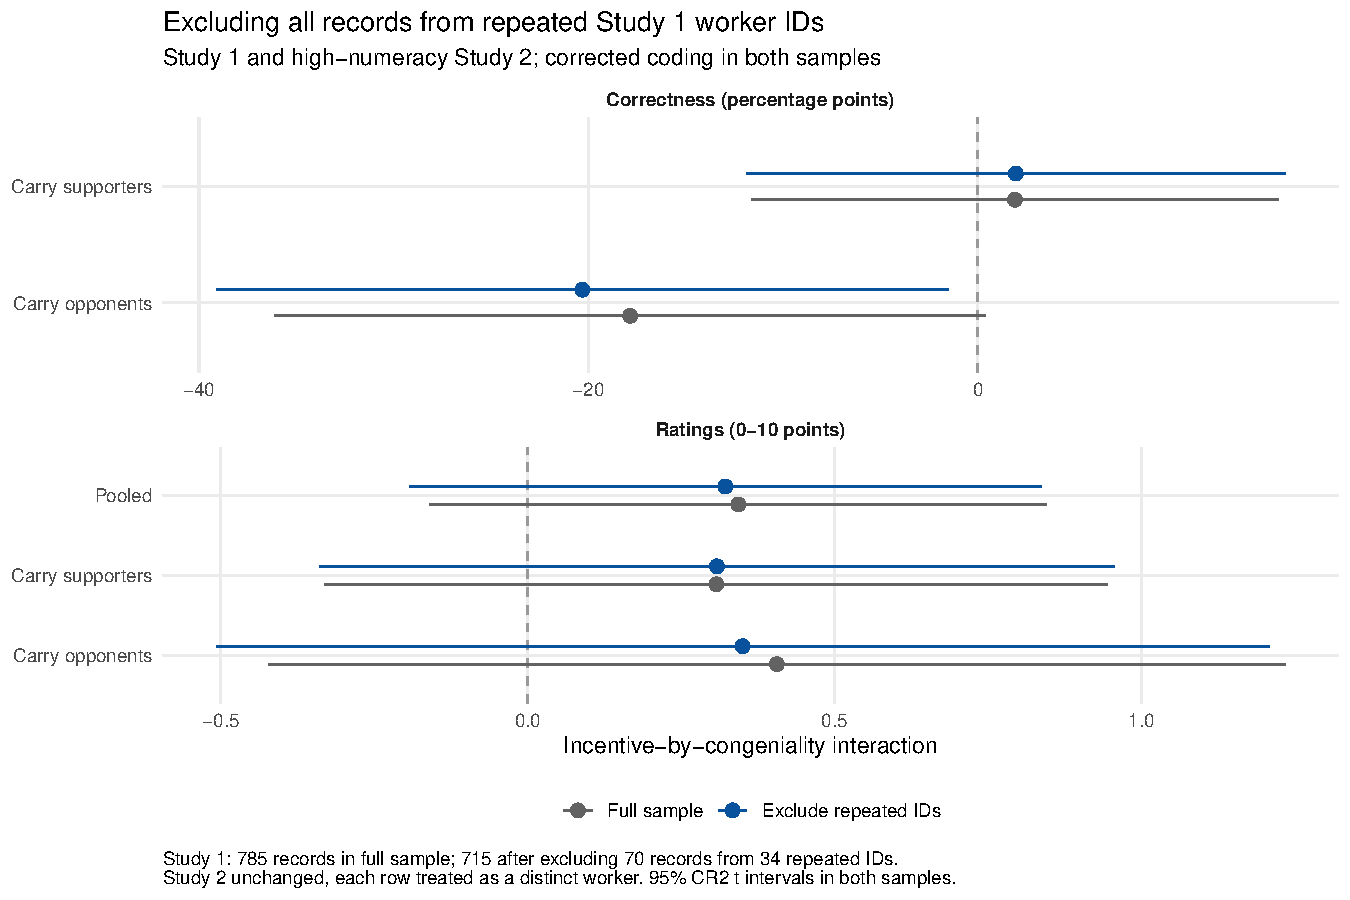
\includegraphics[width=\linewidth]{../figs/worker_exclusion.pdf}
\caption{Incentive-by-congeniality interactions with and without all records from repeated Study 1 worker IDs. Study 2 is restricted to high numeracy and each row is assumed to represent a distinct worker. Both samples use corrected coding and 95\% CR2 t intervals.}\label{fig:worker_exclusion}
\end{figure}
\clearpage
